\clearpage
\VerdierPhysicalPageAnchor{0082}%
\VerdierSemanticAnchor{ch1-3}
\section{Distinguished triangles}

\VerdierSemanticAnchor{ch1-3-1}
\subsection{The cone of a morphism}

\VerdierSemanticAnchor{ch1-3-1-1}
\noindent\textbf{3.1.1.}\quad
\VerdierSemanticAnchor{ch1-3-1-1-tr1-category}
Let $C$ be an additive category. We denote by
$\operatorname{tr}_1(C)$ the following category:

\VerdierSemanticAnchor{ch1-3-1-1-objects}
\noindent--\quad The objects of $\operatorname{tr}_1(C)$ are the morphisms
(of degree zero) $X\xrightarrow{f}Y$ of complexes of objects of $C$.

\VerdierSemanticAnchor{ch1-3-1-1-morphisms}
\noindent--\quad Let $X\xrightarrow{f}Y$ and
$X'\xrightarrow{f'}Y'$ be two objects of $\operatorname{tr}_1(C)$. A morphism
from $X\xrightarrow{f}Y$ to $X'\xrightarrow{f'}Y'$ is a triple
$(g,h,a)$, where $g\colon X\longrightarrow X'$ and
$h\colon Y\longrightarrow Y'$ are morphisms of complexes of degree zero and
where
\VerdierSemanticAnchor{ch1-3-1-1-homotopy-data}
$a\colon f'g\rightsquigarrow hf$ is a homotopy connecting $f'g$ to $hf$.

\VerdierSemanticAnchor{ch1-3-1-1-composition}
\noindent--\quad Let
\begin{equation*}
  \begin{aligned}
    (g,h,a)\colon (X\xrightarrow{f}Y)
      &\longrightarrow (X'\xrightarrow{f'}Y'),\\
    (g',h',a')\colon (X'\xrightarrow{f'}Y')
      &\longrightarrow (X''\xrightarrow{f''}Y'')
  \end{aligned}
\end{equation*}
be two morphisms of $\operatorname{tr}_1(C)$. The composite morphism
\begin{equation*}
  (g'',h'',a'')\colon
  (X\xrightarrow{f}Y)\longrightarrow(X''\xrightarrow{f''}Y'')
\end{equation*}
is then defined by the equalities

\VerdierSemanticAnchor{ch1-3-1-1-eq1}
\begin{equation}
  \begin{aligned}
    g''&=g'g,\\
    h''&=h'h,\\
    a''&=a'\star g+h'\star a.
  \end{aligned}
  \tag{3.1.1.1}
\end{equation}

\VerdierSemanticAnchor{ch1-3-1-1-category-verification}
One immediately verifies that a category has indeed been defined in this way.
\VerdierSemanticAnchor{ch1-3-1-1-diagram-representation}
Most often we shall represent a morphism
$(g,h,a)\colon(X\xrightarrow{f}Y)\longrightarrow
(X'\xrightarrow{f'}Y')$ of $\operatorname{tr}_1(C)$ by a diagram:

\VerdierSemanticAnchor{ch1-3-1-1-eq2}
\begin{equation}
  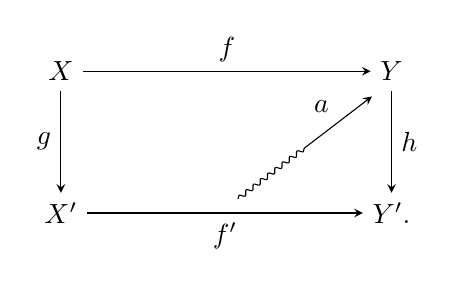
\begin{tikzpicture}[>=stealth,baseline=(current bounding box.center)]
    \node (X)  at (0,1.8) {$X$};
    \node (Y)  at (4.2,1.8) {$Y$};
    \node (Xp) at (0,0) {$X'$};
    \node (Yp) at (4.2,0) {$Y'\mathpunct{.}$};
    \draw[->] (X) -- node[above] {$f$} (Y);
    \draw[->] (X) -- node[left] {$g$} (Xp);
    \draw[->] (Y) -- node[right] {$h$} (Yp);
    \draw[->] (Xp) -- node[below] {$f'$} (Yp);
    \draw[decorate,decoration={snake,amplitude=0.8pt,segment length=3.3pt}]
      (2.25,0.18) -- (3.10,0.83);
    \draw[->] (3.10,0.83) -- node[above left] {$a$} (3.95,1.48);
  \end{tikzpicture}
  \tag{3.1.1.2}
\end{equation}
